\documentclass[12pt]{article}
\usepackage{hyperref}
\usepackage{graphicx}
\usepackage[font=small,labelfont=bf]{caption}
\title{Progetto di fine corso}
\date{17/05/2016}
\author{Alessio Luca,Carlo Sindico}

\begin{document}
	\pagenumbering{arabic}
	
	\begin{titlepage}
		\newcommand{\HRule}{\rule{\linewidth}{0.5mm}}%linea orizzontale
		\center
		
		\textsc{\LARGE Universit\`a degli Studi di Padova}\\[1.5cm] 
		\textsc{\Large Laurea in Informatica}\\[0.5cm]
		\textsc{\large Corso di Tecnologie Web}\\[0.5cm]
		\textsc{\large Progetto di fine corso}\\[0.5cm]
		
		%----------------------------------------------------------------------------------------
		%	TITLE SECTION
		%----------------------------------------------------------------------------------------
		
		\HRule \\[0.4cm]
		{ \huge  2FORCHETTE}\\[0.3cm] 
		\HRule \\[0.4cm]
		
		
		%----------------------------------------------------------------------------------------
		%	AUTHOR SECTION
		%----------------------------------------------------------------------------------------
		
		\begin{minipage}{0.3\textwidth}
			\begin{flushleft} \large
				\emph{Studente:}\\
				Luca \textsc{Alessio} % Your name
			\end{flushleft}
		\end{minipage}
		~
		\begin{minipage}{0.3\textwidth}
			\begin{flushright} \large
				\emph{Matricola:} \\
				\textsc{1070690} % Supervisor's Name
			\end{flushright}
		\end{minipage}\\[2cm]
		
			\begin{minipage}{0.3\textwidth}
				\begin{flushleft} \large
					\emph{Studente:}\\
					Carlo \textsc{Sindico} % Your name
				\end{flushleft}
			\end{minipage}
			~
			\begin{minipage}{0.3\textwidth}
				\begin{flushright} \large
					\emph{Matricola:} \\
					\textsc{1069322} % Supervisor's Name
				\end{flushright}
			\end{minipage}\\[2cm]
			
		%----------------------------------------------------------------------------------------
		%	INFORMATION WEBSITE
		%----------------------------------------------------------------------------------------
		
		\textsc{\Large Informazioni sul sito:}\\[0.3cm]	
		\textsc{http://tecnologie-web.studenti.math.unipd.it/tecweb/~csindico/}\\[1cm]
		
		%----------------------------------------------------------------------------------------
		%	DATI LOGIN
		%----------------------------------------------------------------------------------------
		
			\textsc{\Large Dati login:}\\[0.3cm]
			\textsc{ Username:Admin}\\[0.1mm]
			\textsc{ Password:Admin}\\[0.1mm]
			
		\vfill
	\end{titlepage}
	
	\newpage
	\renewcommand{\contentsname}{Indice}
	\tableofcontents
	
	
	\newpage
	\pagenumbering{arabic}
	
	\section{Abstract}
	\begin{itemize}
		\item Il progetto si propone di offrire  alla maggior parte degli utenti  un sito che ha come contenuto un insieme di ricette. 
			
		Il sito ha un scopo principalmente informativo, infatti riporta tutte le informazioni reltaive a ciascuna ricetta. Le ricette sono classificate in Primi piatti, Secondi piatti, Antipasti e Dessert. L'utente ha la possibilità di proporre una nuova ricetta compilando un apposito form, e un lato amministratore ha il pieno controllo nell'accettare o rifiutare le ricette proposte. Si è trovato utile inserire una sezione commenti, che permette all'utente di chiedere ulteriori informazioni e inviare feedback scrivendo direttamente nel sito, e l'amministratore ha la possibilità di rimuovere i commenti inopportuni.
		
		Il sito è stato creato con lo scopo di essere visualizzato in internet, quindi si è data importanza alla presentazione e alla sua usabilità, rispettando lo standard W3C. Infatti si è data particolare attenzione nella separazione tra struttura presentazione e comportamento con le regole di accessibilità richieste.
	\end{itemize}
		\section{Utenti destinatari}
		\begin{itemize}
			\item Il sito 
		\end{itemize}
		\section{Accessibilit\`a}
		\subsection{Separazione tra struttura,presentazione e comportamento}
		\begin{itemize}
			\item Per una maggiore accessibilità al sito da parte di utenti disabili e per favorire gli algoritmi dei motori di ricerca si è deciso di separarae la struttura dalla presentazione e dal comportamento.
			Infatti il contenuto del sito è rapprentato dai file HTML e CGI, i quali richiamano i fogli di stile CSS e si utilizzano (anche in questo caso attraverso percorsi esterni), esternamente controlli in JavaScript in particolare per la compilazione dei form. Tuttavi il contenuto rimane accessibile anche se JavaScript è disabilitato.(da verificare!!)
			
			Tutto il codice è stato scritto secondo le raccomandazioni W3C,con opportuna validazione di esso.
		\end{itemize}
			\subsection{Colori}
			\begin{itemize}
				\item Si è scelto uno schema di colori non particolarmente vivace (arancione opaco,bianco sporco,nero);Non sono colori di base, ma comunque la lettura dei testi risulta accessibile.Bisogna ricordare che si tratta di un sito di cucina e quindi l'utente si aspetta dei colori vivaci adatti al tipo di sito.(da rivedere!!).Inoltre i link sono sempre sottolineati, e diventano del colore standard quando vengono cliccati.
				Di seguito sono riportate le visualizzazioni del sito attraverso alcuni disturbi visivi:
				
			
			\begin{figure}[ht!]
				\centering
				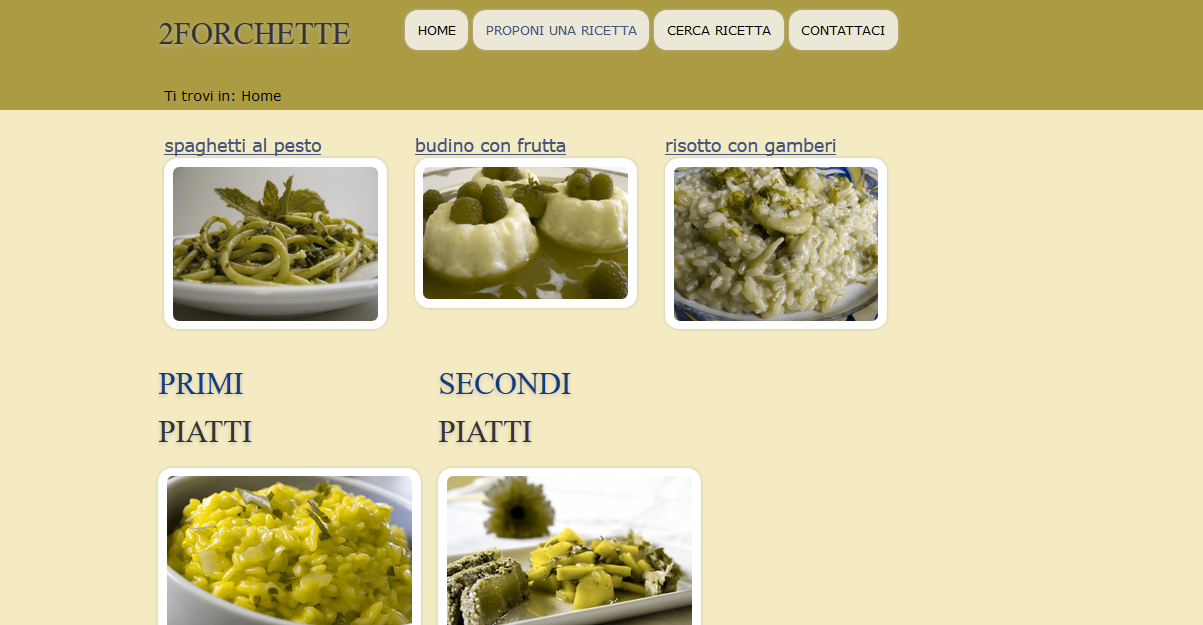
\includegraphics[width=100mm]{test1}
				\caption{vedi file test1.png}
			\end{figure}

				\begin{figure}[ht!]
					\centering
					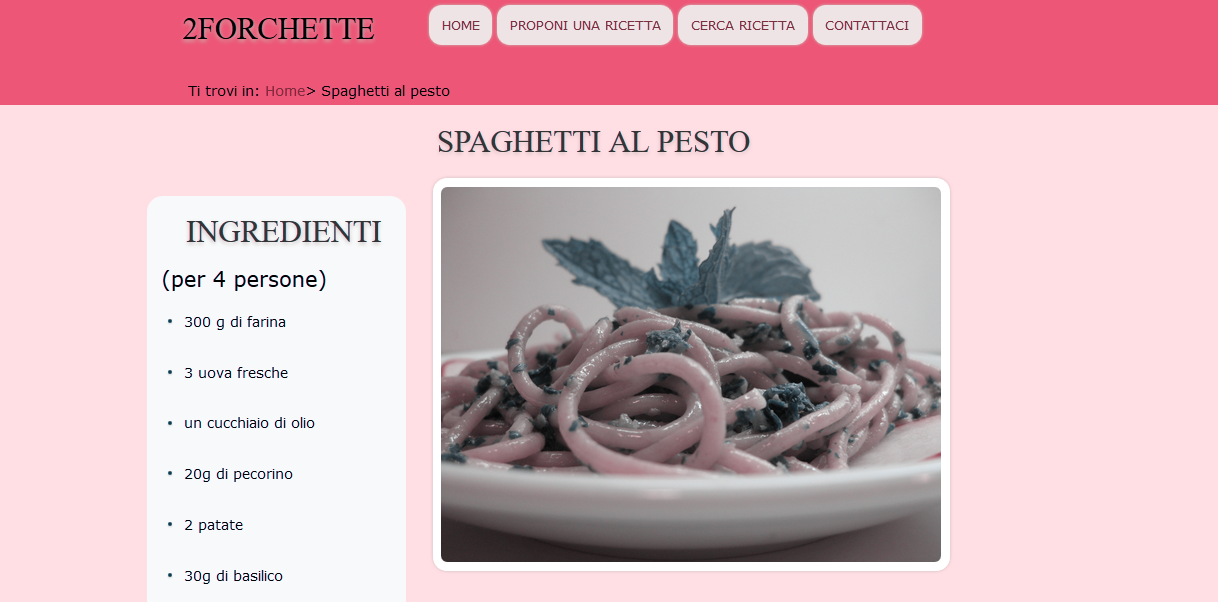
\includegraphics[width=100mm]{test2}
					\caption{vedi file test2.png}
				\end{figure}
			\end{itemize}
			\subsection{Tag meta}
			\begin{itemize}
				\item Sono stati inseriti per ogni pagina i tag meta: title, description,keywords,language,author,content-type.
				il tag title descrive la pagina corrente dal particolare al generale.Il tag description da una descrizione del contenuto del sito, il tag language indica che il sito è stato interamente scritto in italiano. Compaiono però alcune parole inglesi che sono state segnalate agli screenreader attraverso il tag "span xml:lang=en" segnalando la lingua con cui leggere correttamente i vocaboli. 
			\end{itemize}
			\subsection{Screen reader}
			\begin{itemize}
				\item Ogni foto ha il suo attributo alt che descrive ciò che l'immagine ritrae.
				Si è evitato di utilizzare immagini per visualizzare il testo, quindi il contenuto informativo rimane accessibile anche quando fallisce il caricamento delle immagini o del CSS.
			\end{itemize}
			\section{Usabilit\`a}
			\begin{itemize}
				\item Per l'usabilit\`a del sito si è fatta attenzione ad inserire le 6W del giornalismo:
				
				What?: Un utente appena entra nella home capisce subito che si tratta di un sito di ricette, dalla barra dei menù (Proponi ricetta, Cerca ricetta), e dal contenuto in primo piano che mette in evidenza alcune ricette proposte.
				
				Who?: A chi è rivolto il sito? Il sito grazie alle immagini si capisce che è dedicato a mamme e pap\`a
				che vogliono preparare una gustosa ricetta per i propri figli.
				
				Where?: Nonnostante il sito non abbia una propria locazione, già nella home nel footer sono elencati i nomi degli amministratori del sito.Per maggiore visibilit\`a, è stata inserita una pagina CONTATTACI dove oltre ala sezione commenti, sono specificati gli indirizzi email e numero di telefono degli amministratori. 
				
				When?: ..........
				
				Why?: Perchè un utente dovrebbe rimanere nel sito o dovrebbe ritornarci? Il sito è principalmente espositivo,(gli utenti possono liberamente visualizzare le ricette), si è cercato di renderlo più interessante, aggiungendo una sezione proponi ricetta (l'utente ha la possibilità di inserire la propria ricetta), e anche una sezione commenti.
				
				How?: La barra di navigazione mostra tutte le sezioni principali del sito alle quali un utente può accedere.
				
				Nella barra menù è sempre evidenziata la voce della pagina in cui ci troviamo (DA SISTEMARE),e si vede attraverso una diversa colorazione dei link in quali altre pagine si è stati. il testo è sottolineato, per evidenziare il fatto che sono link.
				
				Breadcrumbs: Affinchè l'utente non si perda mai all'interno del sito, è stato ripirtato sotto la barra di navigazione, il percorso che si è effettuato dall'home page.
				
				
			\end{itemize}
			
				
		
	
	
\end{document}